\documentclass[]{article}
\usepackage{lmodern}
\usepackage{amssymb,amsmath}
\usepackage{ifxetex,ifluatex}
\usepackage{fixltx2e} % provides \textsubscript
\ifnum 0\ifxetex 1\fi\ifluatex 1\fi=0 % if pdftex
  \usepackage[T1]{fontenc}
  \usepackage[utf8]{inputenc}
\else % if luatex or xelatex
  \ifxetex
    \usepackage{mathspec}
  \else
    \usepackage{fontspec}
  \fi
  \defaultfontfeatures{Ligatures=TeX,Scale=MatchLowercase}
\fi
% use upquote if available, for straight quotes in verbatim environments
\IfFileExists{upquote.sty}{\usepackage{upquote}}{}
% use microtype if available
\IfFileExists{microtype.sty}{%
\usepackage{microtype}
\UseMicrotypeSet[protrusion]{basicmath} % disable protrusion for tt fonts
}{}
\usepackage[margin=1in]{geometry}
\usepackage{hyperref}
\hypersetup{unicode=true,
            pdftitle={LiDAR-based scaling analysis},
            pdfborder={0 0 0},
            breaklinks=true}
\urlstyle{same}  % don't use monospace font for urls
\usepackage{graphicx,grffile}
\makeatletter
\def\maxwidth{\ifdim\Gin@nat@width>\linewidth\linewidth\else\Gin@nat@width\fi}
\def\maxheight{\ifdim\Gin@nat@height>\textheight\textheight\else\Gin@nat@height\fi}
\makeatother
% Scale images if necessary, so that they will not overflow the page
% margins by default, and it is still possible to overwrite the defaults
% using explicit options in \includegraphics[width, height, ...]{}
\setkeys{Gin}{width=\maxwidth,height=\maxheight,keepaspectratio}
\IfFileExists{parskip.sty}{%
\usepackage{parskip}
}{% else
\setlength{\parindent}{0pt}
\setlength{\parskip}{6pt plus 2pt minus 1pt}
}
\setlength{\emergencystretch}{3em}  % prevent overfull lines
\providecommand{\tightlist}{%
  \setlength{\itemsep}{0pt}\setlength{\parskip}{0pt}}
\setcounter{secnumdepth}{0}
% Redefines (sub)paragraphs to behave more like sections
\ifx\paragraph\undefined\else
\let\oldparagraph\paragraph
\renewcommand{\paragraph}[1]{\oldparagraph{#1}\mbox{}}
\fi
\ifx\subparagraph\undefined\else
\let\oldsubparagraph\subparagraph
\renewcommand{\subparagraph}[1]{\oldsubparagraph{#1}\mbox{}}
\fi

%%% Use protect on footnotes to avoid problems with footnotes in titles
\let\rmarkdownfootnote\footnote%
\def\footnote{\protect\rmarkdownfootnote}

%%% Change title format to be more compact
\usepackage{titling}

% Create subtitle command for use in maketitle
\newcommand{\subtitle}[1]{
  \posttitle{
    \begin{center}\large#1\end{center}
    }
}

\setlength{\droptitle}{-2em}

  \title{LiDAR-based scaling analysis}
    \pretitle{\vspace{\droptitle}\centering\huge}
  \posttitle{\par}
    \author{}
    \preauthor{}\postauthor{}
    \date{}
    \predate{}\postdate{}
  

\begin{document}
\maketitle

\subsection{Empirical scaling versus predicted symmetric
exponents}\label{empirical-scaling-versus-predicted-symmetric-exponents}

Below is a plot of scaling exponents of single trees across the entire
dataset. `Empirical' scaling values along the y-axis are computed via
SMA regressions of subtree volume against the distal number of tips,
which is the essence of understanding how networks supply service
volumes by scaling conduits downward in size. `WBE' scaling values are
computed using the symmetric formula for theta, where whole-tree alpha
and beta values are taken as averages of node-level alpha and beta
values.

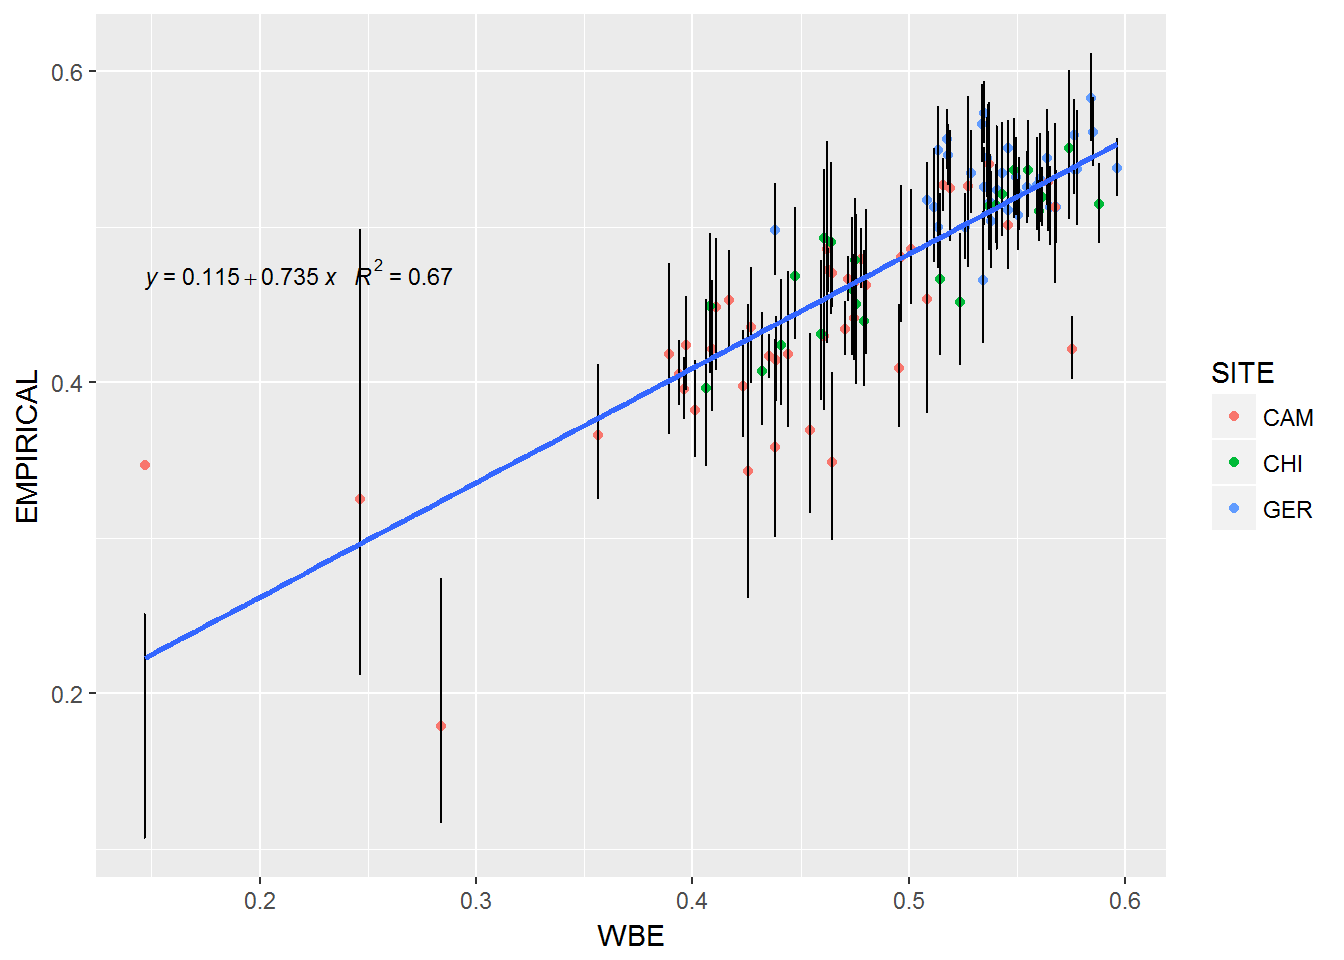
\includegraphics{scaling_report_files/figure-latex/joined_data-1.pdf}

To compute the symmetric exponent using a closed form solution, we
estimated the total number of branching generations for a given network,
N, as log(T)/log(2), where T is the number of terminal elements in the
tree. All scaling theories assume an infinitely large network, and so we
see that `larger' trees tend to approach optimal scaling as well:

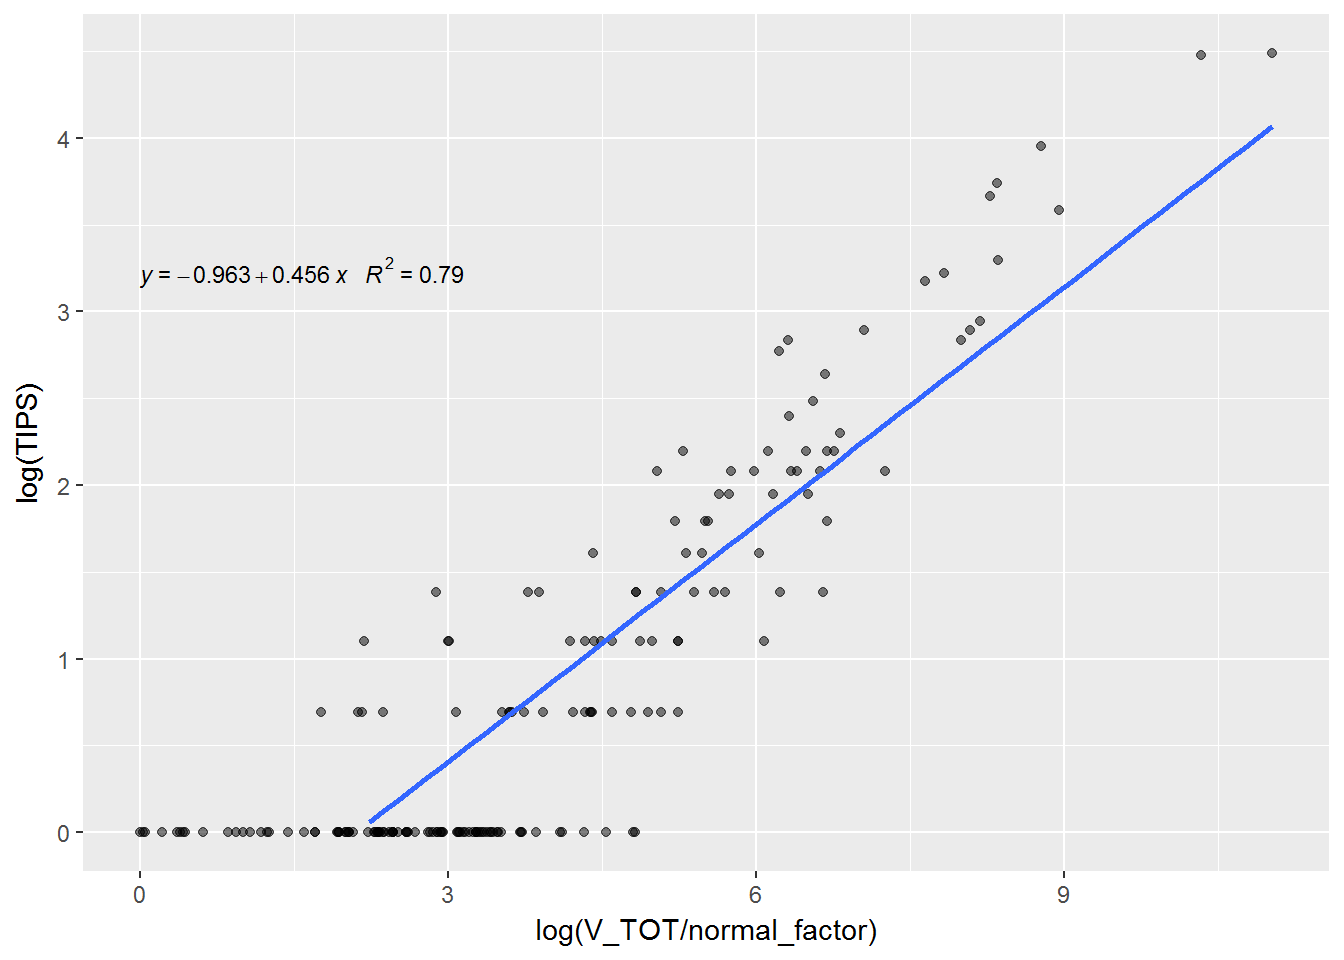
\includegraphics{scaling_report_files/figure-latex/unnamed-chunk-1-1.pdf}

Empirical volume scaling is consistently under-predicted by the
symmetric scaling exponent. Asymmetric scaling theories (Brummer et al
2017) predict that symmetric exponents will fail in most biological
networks. Including asymmetry can lead to positive or negative
deviations from optimal scaling exponents depending on the relative
frequency of asymmetry types. Asymmetry type is decided by the relative
proportions of child branches:

\begin{figure}
\includegraphics[width=9.18in]{figures/brummer_asymmetry} \caption{Two types of asymmetry at the node-level. Figure from Brummer et al 2017}\label{fig:pressure}
\end{figure}

Positive asymmetry leads to volume scaling values between 0.5 and 1,
while negative asymmetry pushes scaling parameters below 0.75. Brummer
et al only derive models of asymmetry for networks assuming one or the
other asymmetry type, acknowledging that empirical networks likely
incorporate both types. Among trees in our dataset, negative asymmetry
appears to be pervasive, which is counter to the expectations of
metabolic scaling theory broadly.

\includegraphics{scaling_report_files/figure-latex/unnamed-chunk-2-1.pdf}

Here, ASYM\_FRAC corresponds to the proportion of nodes in a given tree
displaying positive asymmetry. Thus, for most trees in our dataset,
positive asymmetry exists at a proportion of about 10-40\% of nodes.
Moreover, empirical scaling is clearly negatively correlated with the
frequency of negative asymmetry. Fundamental theory predicts that
negative asymmetry will be selected against because it reduces the
efficiency of metabolic networks (Brummer et al 2017).

There is reason to believe that plant networks, particularly external
architecture represented by branching architecture, should display the
highest proportion of negative asymmetry among biological networks.
Plant crowns are continually exposed to environmental heterogeneity,
causing pruning through a variety of external (disturbance) and internal
(shedding) mechanisms. This pruning is routinely accompanied by dynamic
resprouting via axillary meristem activation.

A heuristic measure of asymmetry, path fraction (Devaud-Smith et al
2014) has been shown to capture some of the functional consequences of
deviation from theoretically optimal scaling parameters. Here we show
the asymmetry proportion against path fraction measured as the average
path length in a tree, divided my the maximum length (Avg L) / (Max L):

\includegraphics{scaling_report_files/figure-latex/unnamed-chunk-3-1.pdf}

Clearly the path fraction is not very sensitive to differences in
positive and negative asymmetry. Moreover, it does not predict variation
in empirical scaling as successfully as the asymmetry fraction:

\includegraphics{scaling_report_files/figure-latex/unnamed-chunk-4-1.pdf}

This indicates the importance of negative asymmetry in driving scaling
patterns across tree species, and may lead to new insights constraining
plant form and function.

Despite the limitations of the symmetrical exponent, scaling results
accord generally with the expectations of functional constraints on
vascular architecture. Below is a plot of symmetric scaling exponents
against wood density, with mean trait values at the genus or family
level when species data is missing from the BIEN database:

\includegraphics{scaling_report_files/figure-latex/unnamed-chunk-5-1.pdf}

Wood density generally decreases as trees get closer to 3/4 scaling.
This is likely due to biomechanical constraints.

Below is a similar plot of leaf area against the predicted symmetric
exponent

\includegraphics{scaling_report_files/figure-latex/unnamed-chunk-6-1.pdf}

Leaf area tends to decrease as trees get closer to 3/4 scaling, which
would likely also correspond to twig size and petiole radius. This
broadly agrees with the body of knowledge surrounding Corner's Rules.


\end{document}
